\documentclass[11pt]{article}
\usepackage[utf8]{inputenc}
\usepackage[T1]{fontenc}
\usepackage[spanish]{babel}
\usepackage{amsmath}
\usepackage{amsfonts}
\usepackage{amssymb}
\usepackage{graphicx}
\usepackage{caption}
\usepackage{wrapfig}
\usepackage{subcaption}
\usepackage{textcomp}
\usepackage{siunitx}
\usepackage{geometry}
\usepackage{courier}
\usepackage{cancel}
\spanishdecimal{.}

\title{Física Numérica}
\author{Julio César Avila Torreblanca}
\date{09 de noviembre del 2021}

\setlength{\parindent}{0cm}
\geometry{verbose,tmargin=1in,bmargin=1in,lmargin=1in,rmargin=1in}
\begin{document}
	\maketitle
	
\section*{Tarea 6}
%%%%%%%%%%%%%%%%%%%%%%%%%%%%%%%%%%%%%%%%%%%%%%%%%%%%%%%%%%%%%%%%%%%%%%%%%%%%%%%%%%%%%%%%%%%%%%%%%%%%%%%%%%%%%%%%%%%%%%%%	
\subsection*{\textbf{1. Interpolación de Lagarange}}
%%%%%%%%%%%%%%%%%%%%%%%%%%%%%%%%%%%%%%%%%%%%%%%%%%%%%%%%%%%%%%%%%%%%%%%%%%%%%%%%%%%%%%%%%%%%%%%%%%%%%%%%%%%%%%%%%%%%%%%%
	\begin{enumerate}
		\item [\textbf{(a)}]Escriba un programa que ajuste un polinomio según el algoritmo de Lagrange a un conjunto de $n$ puntos.
	\end{enumerate}
	\textit{Solución.}\\
		Aquí haremos uso de las siguientes librerías.
		%%%Librerías
		\begin{figure}[h]
			\centering
			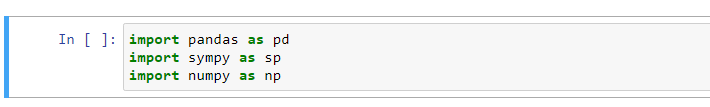
\includegraphics[width=12cm]{Img/1a1.PNG}
		\end{figure}
		Recordemos que en el algoritmo de interpolación de Lagrange, tenemos una variable independiente $x$ y $n$ valores de ella: $x_i$ ($i=1,2,...,n$). Para esta variable independiente existe una función $g(x)$ con valores $g_i = g(x_i)$. Con esto se busca aproximar a $g(x)$ mediante un polinomio de grado $n-1$, dado por:
		\begin{equation}\label{Pol Lagrange}
			g(x) \approx \sum_{i=1}^{n} g_i L_i(x)		
		\end{equation}
		Donde:
		\begin{equation} \label{coeicientes}
			L_i(x) = \prod_{j(\neq i)=1}^{n} \frac{x-x_j}{x_i - x_j} = \frac{x-x_1}{x_i -x_1} \frac{x-x_2}{x_i -x_2} \cdots \frac{x-x_n}{x_i -x_n} 
		\end{equation}
		Con base en esto, crearemos un algoritmo que realice interpolación de Lagrange.\\
		
		Lo primero que haremos será crear una función llamada \texttt{Lx}, la cual calculará los polinomios $L_i(x)$ usando la ecuación (\ref{coeicientes}). Notemos que estos polinomios son de grado $n-1$. Para esta función nos apoyaremos del cálculo simbólico integrado por la librería \texttt{sympy}. Como parámetros se piden el subíndice \texttt{i} del polinomio $L_i(x)$ por calcular y una lista \texttt{values} que contendrá los datos conocidos de la variable independiente $x$: $(x_1,x_2,..., x_n)$.
		
		El código de la función es el siguiente (los comentarios contienen una explicación de qué se está realizando en cada sentencia):
\newpage
		\begin{figure}[h]
			\centering
			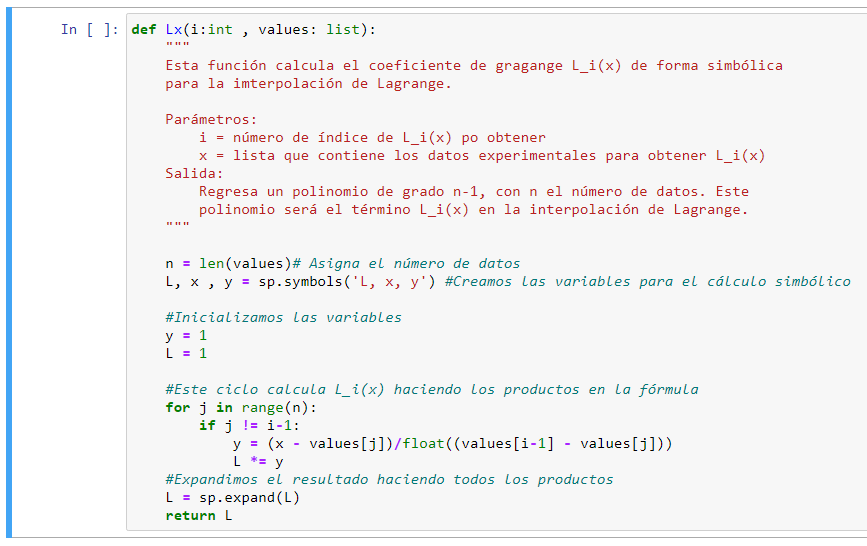
\includegraphics[width=15cm]{Img/1a2.PNG}
		\end{figure}
	
	Ya con esta función será muy sencillo calcular el polinomio de Lagrange a partir de la fórmula (\ref{Pol Lagrange}) y completar el algoritmo para realizar interpolación de Lagrange.\\
	Dentro del código debemos importar los datos experimentales usando la librería \texttt{pandas}. Ya con esos datos, guardaremos los puntos de interés $(x_1,x_2,...,x_n)$ y $(g_1,g_2,...,g_n)$ en dos arreglos distintos. Para no tener problemas con el manejo de estos datos, los transformaremos en tipo \texttt{float64}. Después guardaremos en una variable \texttt{n} el número de datos que coincide con la longitud de cualquier arreglo, esto es necesario saber ya que en la fórmula (\ref{Pol Lagrange}) se necesita. Enseguida definimos las variables simbólicas \texttt{g} y \texttt{x} para obtener $g(x)$ a través del cálculo simbólico usando \texttt{sympy}. Por último, a través de un ciclo \texttt{for} haremos los cálculos correspondientes a la fórmula (\ref{Pol Lagrange}) para generar nuestro polinomio $g(x)$. Este proceso se aprecia en el siguiente código: 
	\begin{figure}[h]
		\centering
		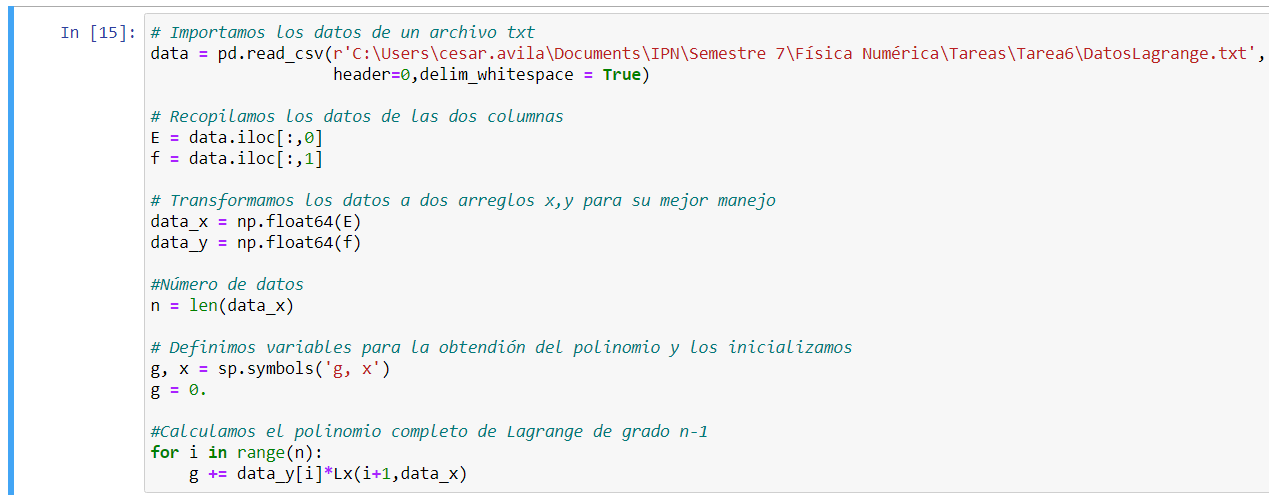
\includegraphics[width=17cm]{Img/1a3.PNG}
	\end{figure}
	
	El código anterior calcula el polinomio de Lagrange para cualquier conjunto de $n$ puntos, solo hace falta cambiar la ruta del archivo en el renglón 2 por el archivo que se desee. En este caso hemos usado la ruta del archivo que se pide en el siguiente inciso. Lo único que resta es poner aprueba el algoritmo y graficar para ver el resultado. Esto se hará en el siguiente inciso.
	
%%%%%%%%%%%%%%%%%%%%%%%%%%%%%%%%%%%%%%%%%%%%%%%%%%%%%%%%%%%%%%%%%%%%%%%%%%%%%%%%%%%%%%%%%%%%%%%%%%%%%%%%%%%%%%%%%%%%%%%%%	
	\begin{enumerate}
		\item [\textbf{(b)}]Utilice su programa para ajustar un polinomio al conjunto de datos:
			\begin{figure}[h]
			\centering
			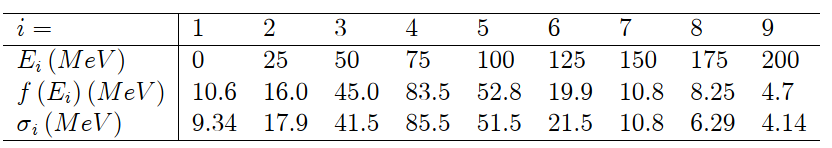
\includegraphics[width=12cm]{Img/datos1.PNG}
		\end{figure}
		Utilice si ajuste para graficar la sección eficaz en pasos de 5 MeV
	\end{enumerate}
	\textit{Solución.}\\
	Primeramente creamos un archivo .txt que contenga los datos experimentales. Estos datos los leemos con el algoritmo del inciso anterior para generar el polinomio de Lagrange correspondiente. El polinomio generado para estos datos es el siguiente:
	\begin{figure}[h]
		\centering
		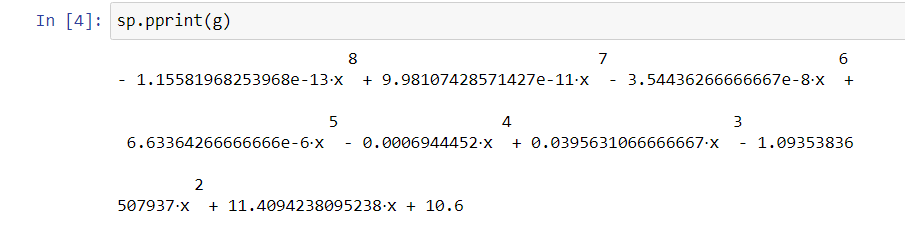
\includegraphics[width=12cm]{Img/1a4.PNG}
	\end{figure}
	
	Lo siguiente a realizar es graficar este polinomio junto con los datos experimentales para hacer la comparación y evaluar el ajuste obtenido.\\
	Para esta parte usaremos las siguientes librerías.
	\begin{figure}[h]
		\centering
		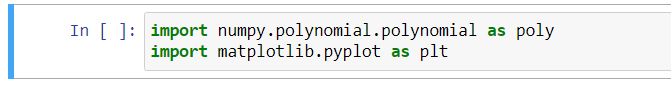
\includegraphics[width=12cm]{Img/1a5.PNG}
	\end{figure}
	
	En el algoritmo primero convertimos el polinomio \texttt{g} a un objeto tipo polinomio de la librería de \texttt{numpy} y extraemos los coeficientes en un arreglo llamado \texttt{coef}. Luego reacomodamos los coeficientes para crear el polinomio adecuado en una variable llamada \texttt{pol}. Enseguida creamos un arreglo llamado \texttt{valores\_E} que contendrá los puntos a ser evaluados en el eje $x$, notemos que en la definición de este arreglo contendrá la longitud de los pasos de 5 MeV que se piden. Lo siguiente a realizar es definir la gráfica y evaluar en los puntos que se tienen. Esto se observa en el siguiente algoritmo:
\newpage
	\begin{figure}[h]
		\centering
		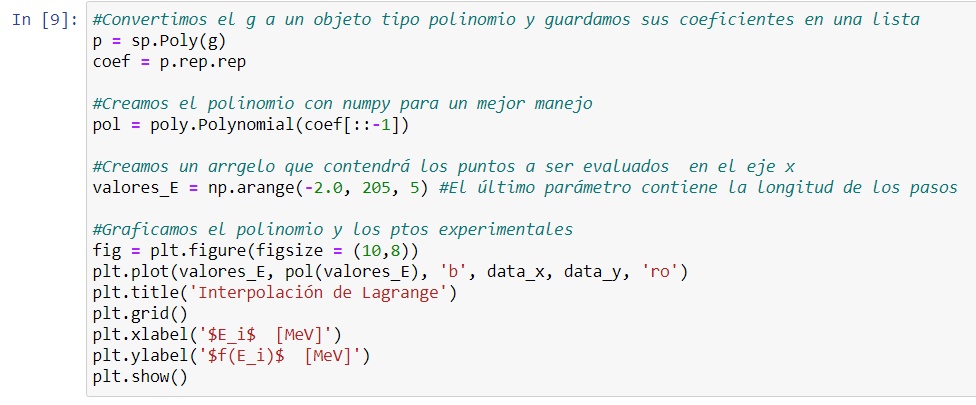
\includegraphics[width=16cm]{Img/1a6.PNG}
	\end{figure}
	
	A partir de esto generamos el siguiente gráfico donde la recta azul muestra el polinomio de Lagrange obtenido y los puntos rojos son los puntos experimentales.
	\begin{figure}[h]
		\centering
		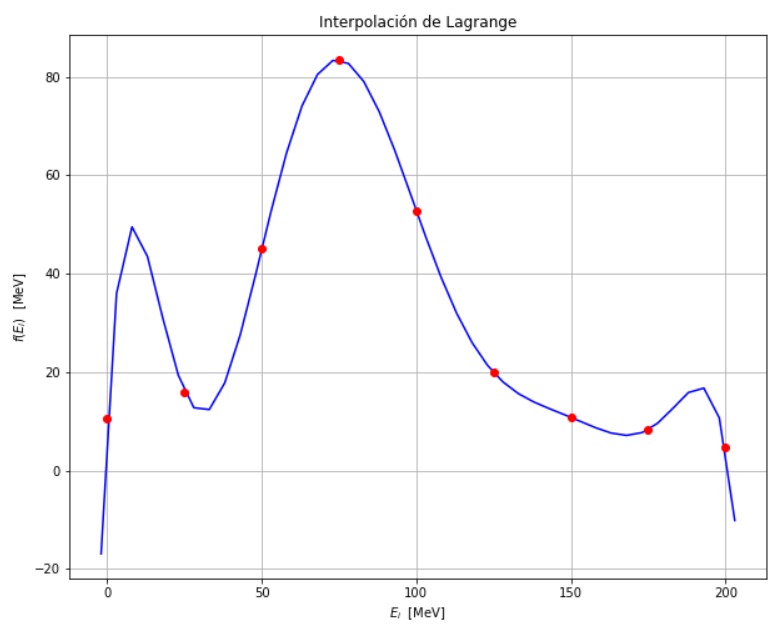
\includegraphics[width=11cm]{Img/1a7.PNG}
		\caption{Gráfica del polinomio de Lagrange con pasos de 5 MeV.}
		\label{Lagrange}
	\end{figure}
	
	El polinomio de Lagrange pasa por todos los puntos experimentales. La razón por la que las curvas no son suaves es porque se graficó en pasos de 5 MeV. Si se hace más pequeño el paso, se tendrán curvas más suaves. Por último, notemos que este tipo de ajuste, a pesar de que pasa por todos los puntos, no es correcto. Esto se debe a que hay zonas donde se crean picos o curvas que se desvían de la tendencia y no nos dicen nada en esa sección. Por lo que este método no es adecuado para ajustar nuestros datos.
	
	
	
%%%%%%%%%%%%%%%%%%%%%%%%%%%%%%%%%%%%%%%%%%%%%%%%%%%%%%%%%%%%%%%%%%%%%%%%%%%%%%%%%%%%%%%%%%%%%%%%%%%%%%%%%%%%%%%%%%%%%%%%
	\begin{enumerate}
		\item [\textbf{(c)}]Utilice su gráfica para estimar la energía de resonancia $E_r$ y $\Gamma$ el ancho a la mitad del máximo (\textit{full-width at half-maximun}). Compare sus resultados con el valor predicho por la teoría $(E_r,\Gamma) = (\SI{78}{MeV}, \SI{55}{MeV})$.
	\end{enumerate}
	\textit{Solución.}\\
	Para obtener la energía de resonancia, necesitamos el máximo absoluto de nuestro polinomio de Lagrange. Notemos que este punto está cercano al punto experimental rojo con $f(E_i) = 75$ MeV. Para determinar$E_r$, realizaremos el criterio de la primera derivada y obtendremos las raíces del polinomio resultante. Estas raíces serán los candidatos a ser máximos o mínimos, y como sabemos que el máximo absoluto es cercano a $f(E_i) = 75 \,\,\si{MeV}$, tomaremos la raiz más cercana a ese valor.\\
	En el siguiente algoritmo se realiza esta parte:
	\begin{figure}[h]
		\centering
		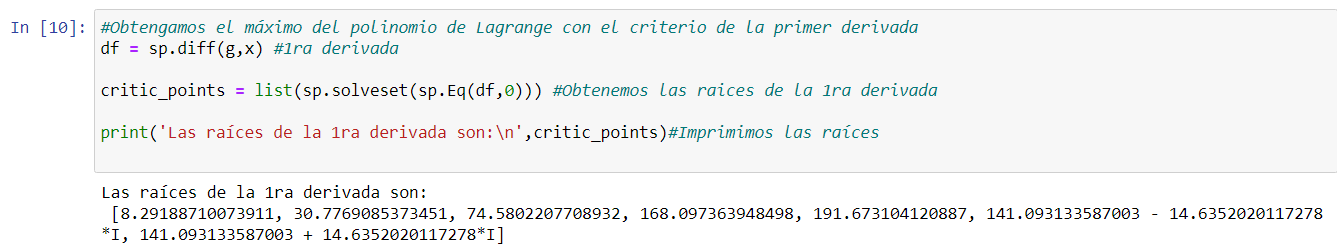
\includegraphics[width=17cm]{Img/1a8.PNG}
	\end{figure}
	
	Notemos que el valor buscado está en la posición 2 de la lista. Así nuestra energía de resonancia para el polinomio de Lagrange obtenido está dada por:
	$$E_r = \SI{74.5802207708932}{MeV}$$
	Por otro lado, para determinar $\Gamma$ basta resolver la ecuación $g(x)=\frac{g(E_r)}{2}$, donde $g(x)$ es el polinomio de Lagrange. Si analizamos la figura (\ref{Lagrange}), las dos soluciones que nos interesan deben ser las más cercanas a la energía de resonancia $E_r$. La diferencia de estos dos valores será el valor de $\Gamma$. En el siguiente código se muestra este proceso.
	\begin{figure}[h]
		\centering
		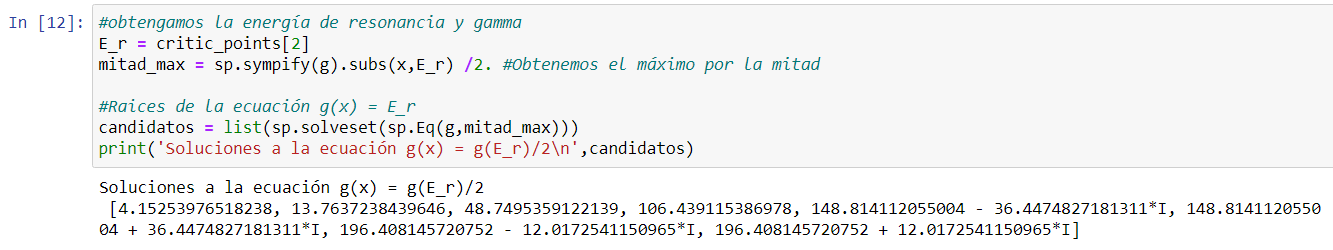
\includegraphics[width=15cm]{Img/1a9.PNG}
	\end{figure}

	Los valores que nos interesan son los elementos en las posiciones 2 y 3 de la lista. Así la diferencia de estos nos da el valor de $\Gamma$.
	\begin{figure}[h]
		\centering
		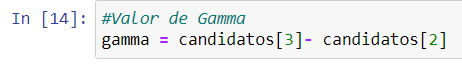
\includegraphics[width=10cm]{Img/1a10.PNG}
	\end{figure}
	
	Comparando con los valores teóricos tenemos los siguientes resultados:
\newpage
	\begin{figure}[h]
		\centering
		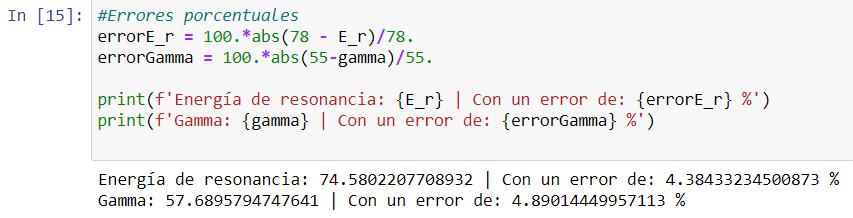
\includegraphics[width=13cm]{Img/1a11.PNG}
	\end{figure}
	
	Podemos ver que los valores que se determinaron para $E_r$ y $\Gamma$ son muy cercanos a los valores teóricos.\\
	
%%%%%%%%%%%%%%%%%%%%%%%%%%%%%%%%%%%%%%%%%%%%%%%%%%%%%%%%%%%%%%%%%%%%%%%%%%%%%%%%%%%%%%%%%%%%%%%%%%%%%%%%%%%%%%%%%%%%%%%%	
\hrule
\subsection*{\textbf{2. Interpolación vía splines cúbicos}}

%%%%%%%%%%%%%%%%%%%%%%%%%%%%%%%%%%%%%%%%%%%%%%%%%%%%%%%%%%%%%%%%%%%%%%%%%%%%%%%%%%%%%%%%%%%%%%%%%%%%%%%%%%%%%%%%%%%%%%%%
\begin{enumerate}
	\item [\textbf{(a)}] Para los datos del problema anterior, ajuste splines cúbicos utilizando una rutina de las bibliotecas de Python. Estime los valores para la energía de resonancia $E_r$ y $\Gamma$ el ancho a la mitad del máximo (\textit{full-width at half-maximum}).
\end{enumerate}
	\textit{Solución.}\\
	Para este ejercicio utilizaremos la rutina \texttt{CubicsSpline} de la librería de \texttt{scipy}. En el siguiente algoritmo se crea el spline cúbico. Al igual contiene comentarios que explican que hace cada parte.
	\begin{figure}[h]
		\centering
		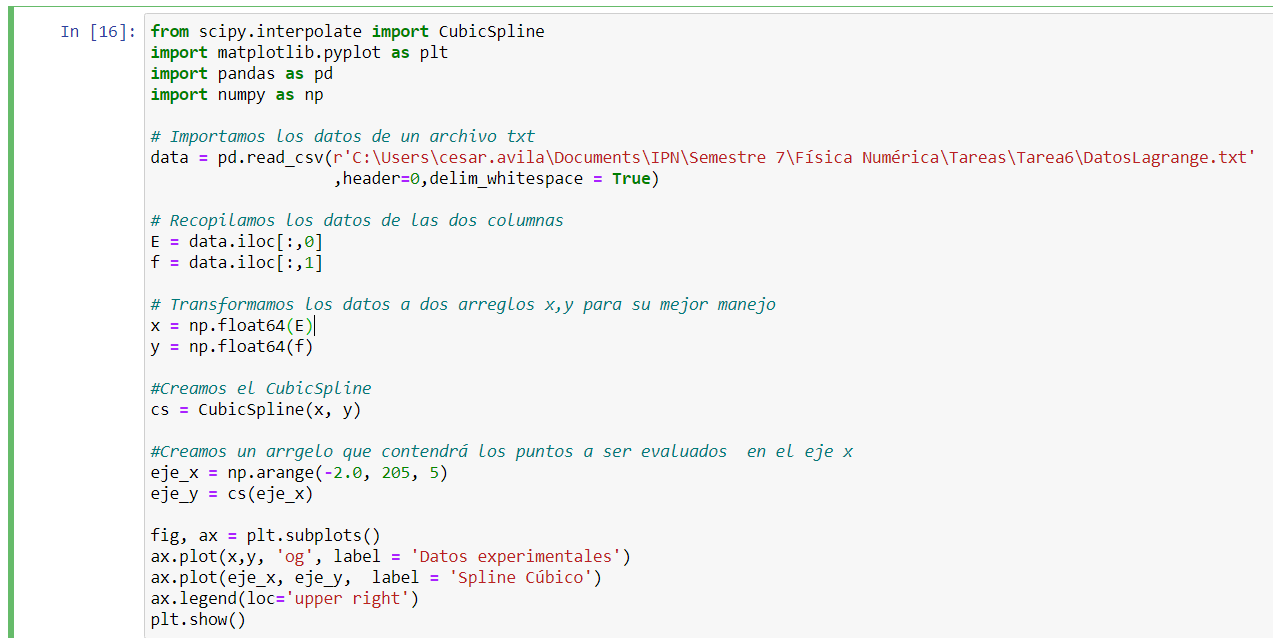
\includegraphics[width=16cm]{Img/2a1.PNG}
	\end{figure}

	El ajuste obtenido fue el siguiente:
\newpage

	\begin{figure}[h]
		\centering
		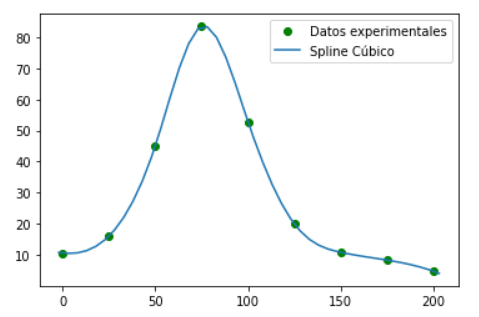
\includegraphics[width=12cm]{Img/2a2.PNG}
		\caption{Ajuste por Splines Cúbicos con pasos de 5 MeV.}
	\end{figure}
	
	Podemos apreciar que este ajuste es mucho mejor que la interpolación de Lagrange, pues se aproxima mejor a la tendencia de los datos.\\
	Para determinar el valor de la energía de resonancia, usaremos un \texttt{while} en el cual se evaluará de 1 en 1 nuestro ajuste $g(x)$ de Spline Cúbico y guardará el valor $x_0$ para el cual $g(x_0)$ es máxima. Esto se aprecia en el siguiente algoritmo: 
	\begin{figure}[h]
		\centering
		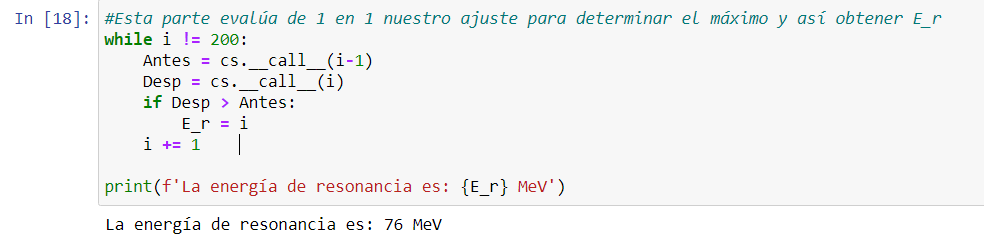
\includegraphics[width=13cm]{Img/2a4.PNG}
	\end{figure}

	Por lo tanto, para el ajuste por Spline Cúbicos obtenemos:
	$$E_r = \SI{76}{MeV}$$
	
	Ahora para determinar Gamma recorreremos nuestro spline cúbico en el eje $y$ el valor de la mitad del máximo y obtendremos las raíces. Esto se realiza en el siguiente algoritmo:
\newpage	
	\begin{figure}[h]
		\centering
		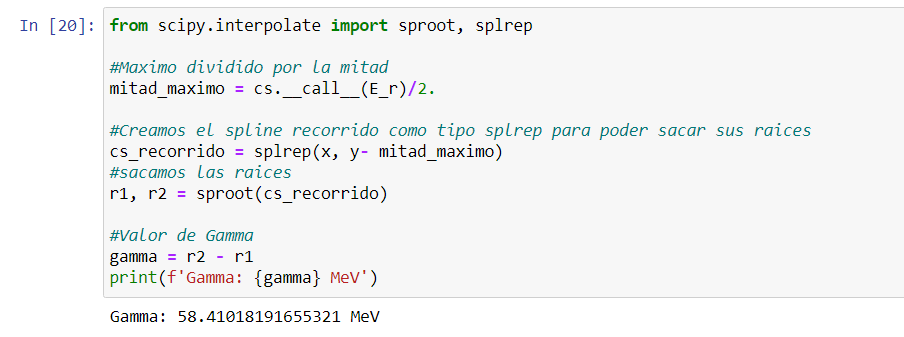
\includegraphics[width=13cm]{Img/2a5.PNG}
	\end{figure}

	Cuando se recorre nuestro spline cúbico se obtiene lo siguiente:
	\begin{figure}[h]
		\centering
		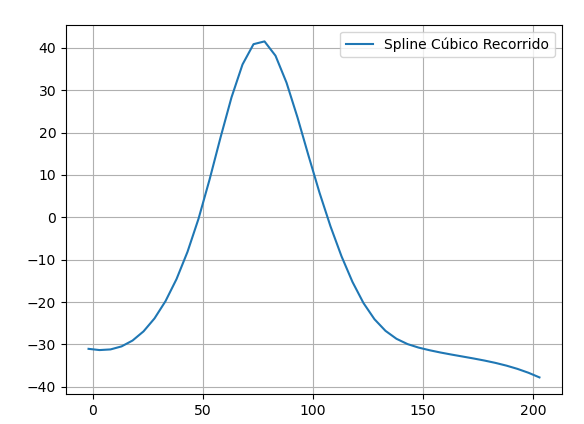
\includegraphics[width=8cm]{Img/2a3.PNG}
		\caption{Spline Cúbico recorrido.}
	\end{figure}

	Notemos que las raíces reales serán los valores que determinarán $\Gamma$. El valor obtenido fue $\Gamma = \SI{58.41018191655321}{MeV}$.\\
	Comparando con los valores teóricos tenemos los siguientes resultados:
	\begin{figure}[h]
		\centering
		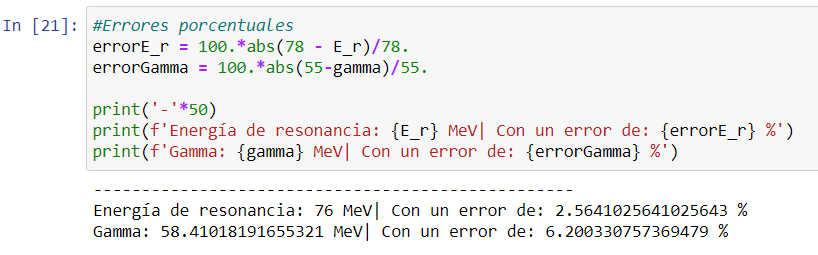
\includegraphics[width=13cm]{Img/2a6.PNG}
	\end{figure}
%%%%%%%%%%%%%%%%%%%%%%%%%%%%%%%%%%%%%%%%%%%%%%%%%%%%%%%%%%%%%%%%%%%%%%%%%%%%%%%%%%%%%%%%%%%%%%%%%%%%%%%%%%%%%%%%%%%%%%%%	
\hrule

\subsection*{\textbf{3. Ajuste de la fórmula de resonancia de Breit-Wigner}}

%%%%%%%%%%%%%%%%%%%%%%%%%%%%%%%%%%%%%%%%%%%%%%%%%%%%%%%%%%%%%%%%%%%%%%%%%%%%%%%%%%%%%%%%%%%%%%%%%%%%%%%%%%%%%%%%%%%%%%%%
\begin{enumerate}
	\item [\textbf{(a)}] Para la teoría indica que la fórmula de Breit - Wigner  debe ajustar a los datos de los dos ejercicios anteriores:
	\begin{equation}\label{Breit}
		f(E) = \frac{f_r}{(E - E_r)^2 + \frac{\Gamma^2}{4}}
	\end{equation}
	Su problema consiste en determinar los valores para los parámetros $E_r$, $f_r$ y $\Gamma$. Se sugiere renombrar los parámetros haciendo:
	$$a_1 = f_r,\quad a_2= E_r, \quad a_3 = \frac{\Gamma^2}{4},\quad x=E$$
	Para escribir:
	\begin{equation}\label{xi}
		g(x) =\frac{a_1}{(x-a_2)^2 + a_3}
	\end{equation}
	y encontrar los parámetros a partir de minimizar $\chi^2$, encuentre estas ecuaciones.
\end{enumerate}
\textit{Solución.}\\
	Las ecuaciones que minimizan a $\chi^2$ son: 
	\begin{eqnarray}
		f_1(a_1, a_2, a_3) &=& \sum_{i=1}^{9} \dfrac{y_i - g(x_i)}{\left[ (x_i - a_2)^2 + a_3\right] \sigma_i^2} = 0  \\
		f_1(a_1, a_2, a_3) &=& \sum_{i=1}^{9} \dfrac{(y_i - g(x_i)) (x_i - a_2)}{\left[ (x_i - a_2)^2 + a_3\right]^2 \sigma_i^2} = 0  \\
		f_1(a_1, a_2, a_3) &=& \sum_{i=1}^{9} \dfrac{(y_i - g(x_i))}{\left[ (x_i - a_2)^2 + a_3\right]^2 \sigma_i^2} = 0  
	\end{eqnarray}

	Obtengamos estas ecuaciones en python. Para ello usemos las siguientes librerías:
	\begin{figure}[h]
		\centering
		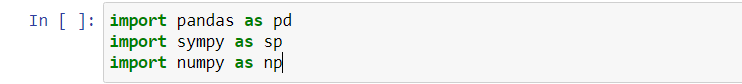
\includegraphics[width=12cm]{Img/3a1.PNG}
	\end{figure}

	Para generar $g(x)$ crearemos la siguiente función:
	\begin{figure}[h]
		\centering
		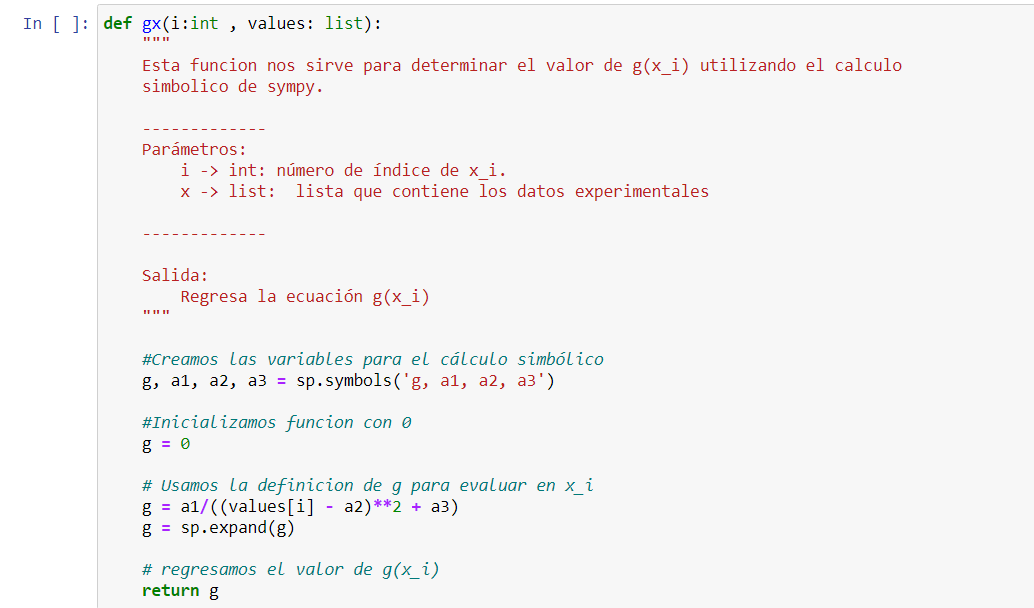
\includegraphics[width=13cm]{Img/3a2.PNG}
	\end{figure}
	
	Ya con esta función podremos generar las funciones $f_1,f_2,f_3$. Primeramente leamos los datos experimentales y transformemoslos a flotantes:
\newpage	
	\begin{figure}[h!]
		\centering
		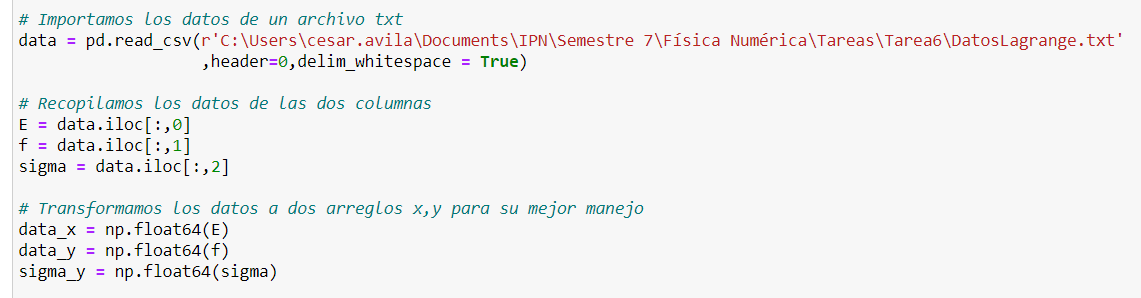
\includegraphics[width=15cm]{Img/3a3.PNG}
	\end{figure}

	Ya con esto definamos las variables simbólicas con la librería de \texttt{sympy} y calculemos las funciones $f_1, f_2, f_3$.
	
	\begin{figure}[h!]
		\centering
		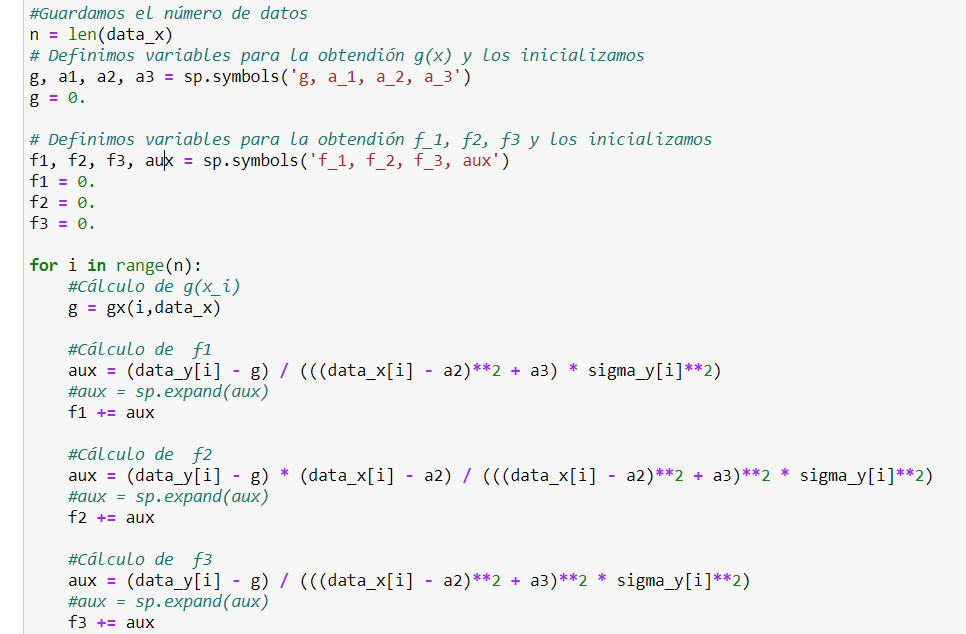
\includegraphics[width=15cm]{Img/3a4.PNG}
	\end{figure}



\begin{enumerate}
	\item [\textbf{(b)}] Las ecuaciones que obtuvo en el inciso anterior NO son lineales, elabore un programa que utilice el método de Newton-Raphson
	multidimensional para la búsqueda de raíces.
\end{enumerate}
\textit{Solución.}\\
	Las semillas que usaremos para el método de Newton-Raphson serán los valores teóricos del ejercicio 1 : $(E_r,\Gamma) = (\SI{78}{MeV}, \SI{55}{MeV})$. Esto con el objetivo de acelerar la convergencia.
	
	\begin{figure}[h]
		\centering
		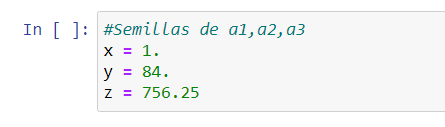
\includegraphics[width=8cm]{Img/3b1.PNG}
	\end{figure}
	
	EL método de Newton-Raphson de forma multidimensional, nos dice que dado un vecor de funciones $\vec{f}$ el cual tiene por entradas a las funciones $f_i$ determinadas en el inciso (a), se cumple lo siguiente:
	$$\vec{f}  + \vec{J} \Delta \vec{x} = 0$$
	
	Donde $\vec{J}$ es la matriz jacobiana de las $f_i$'s y $\Delta \vec{x}$  es el vector de los desplazamientos que se realizan con este algoritmo. De esta forma, encontraremos una solución de la forma:
		$$ \Delta \vec{x} =  - \vec{J}^{\prime - 1} \vec{f}$$
	Este proceso se realiza en el siguiente código:\\
	Primero definimos las funciones que nos generarán las matrices $\vec{f}$ y la matriz jacobiana $\vec{J}$.
	\begin{figure}[h]
		\centering
		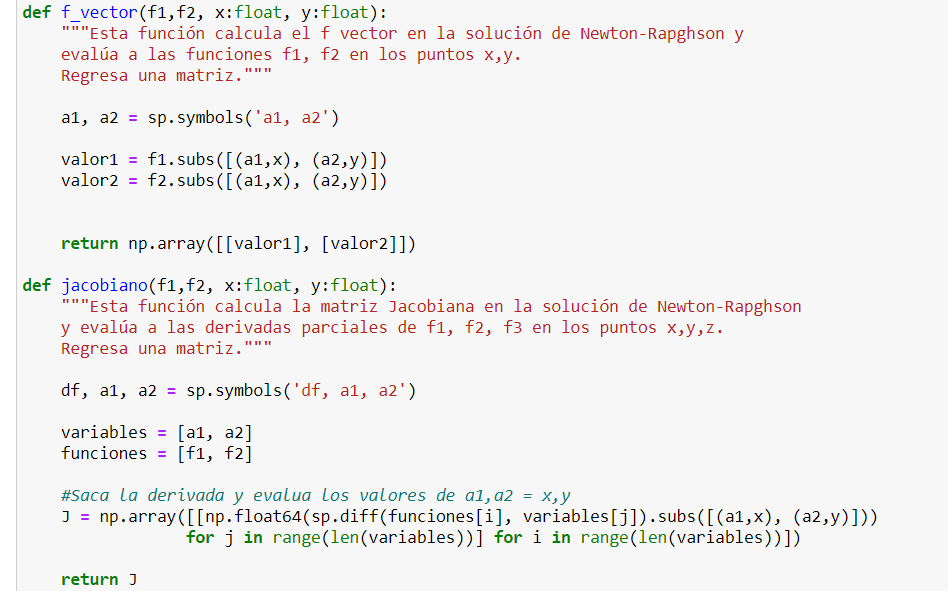
\includegraphics[width=14cm]{Img/3b2.PNG}
	\end{figure}
	
	Luego definamos las siguientes variables que nos ayudaran a realizar las iteraciones para Newton-Raphson:
	\begin{figure}[h]
		\centering
		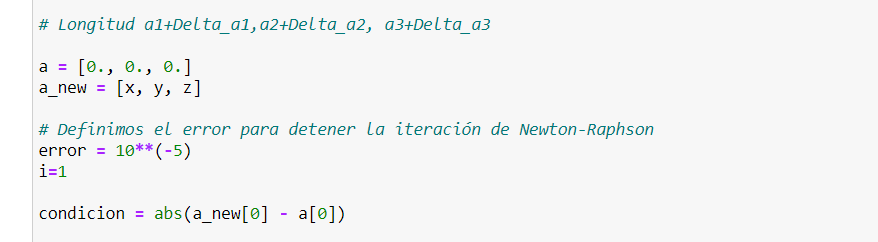
\includegraphics[width=13cm]{Img/hhh.PNG}
	\end{figure}
\newpage
Ya con las matrices definidas, podremos iterar para obtener las estimaciones para $a_1,a_2,a_3$. 

\begin{figure}[h]
	\centering
	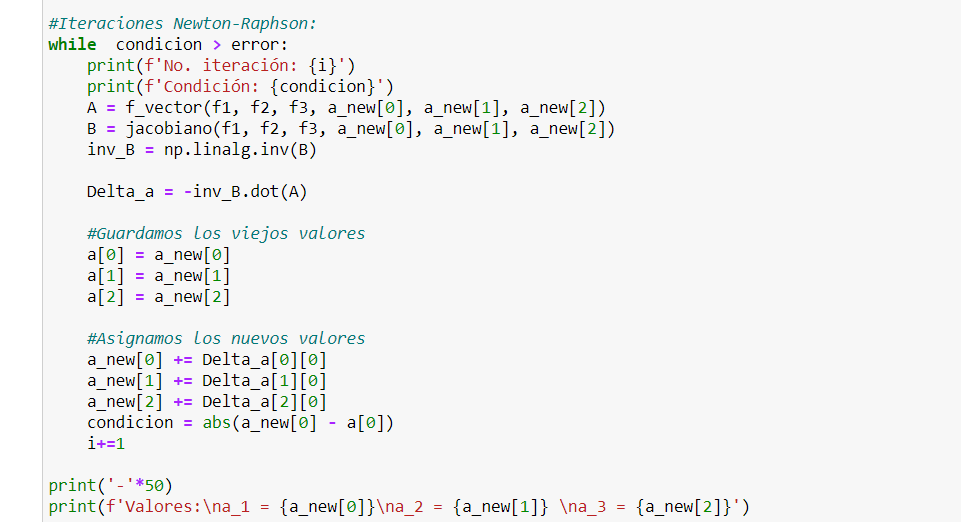
\includegraphics[width=14cm]{Img/w.PNG}
\end{figure}

El código anterior nos produce los siguientes resultados:
\begin{figure}[h]
	\centering
	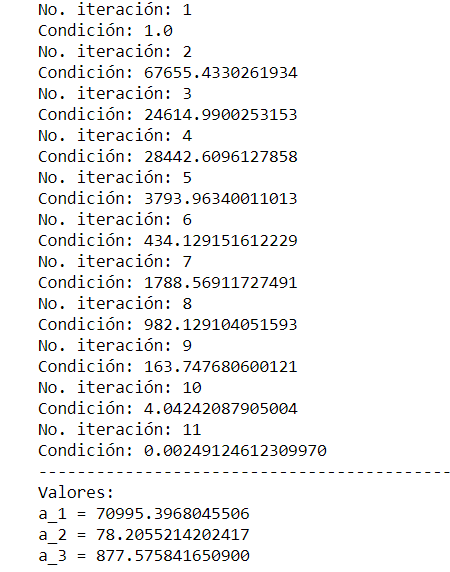
\includegraphics[width=7cm]{Img/3b4.PNG}
\end{figure}
\hrule
	\newpage
%%%%%%%%%%%%%%%%%%%%%%%%%%%%%%%%%%%%%%%%%%%%%%%%%%%%%%%%%%%%%%%%%%%%%%%%%%%%%%%%%%%%%%%%%%%%%%%%%%%%%%%%%%%%%%%%%%%%%%%%	

\subsection*{\textbf{4. Decaimiento de una fuente de voltaje}}

%%%%%%%%%%%%%%%%%%%%%%%%%%%%%%%%%%%%%%%%%%%%%%%%%%%%%%%%%%%%%%%%%%%%%%%%%%%%%%%%%%%%%%%%%%%%%%%%%%%%%%%%%%%%%%%%%%%%%%%%
Cuando una fuente de voltaje se conecta a tavés de una resistencia y un inductor en serie, el voltaje a trabés del inductor $V_i(t)$ obedece la ecuación:
\begin{align}
	V(t) = V_0 e^{-\Gamma t}	\label{voltaje}
\end{align}
donde $t$ es el tiempo y $\Gamma = \frac{R}{L}$ es el cociente de la resistencia $R$ y la inductancia $L$ del circuito. Con base en los datos experimentales:
\begin{enumerate}
	\item [\textbf{(a)}] Encuentre el mejor estimado para los valores de $\Gamma$ y $V_0$.
\end{enumerate}
\textit{Solución.}\\
	Sea $a_1 = V_0$ y $a_2 = \Gamma$. Así nuestra ecuación para hacer ajuste por mínimos cuadrados resulta:
	\begin{equation}
		g(t) = a_1 e^{-a_2 t}	\label{hh}
	\end{equation}
	Luego:
	\begin{align*}
		\frac{\partial g}{\partial a_1} & = e^{-a_2 t}	\\
		 \frac{\partial g}{\partial a_2} & = -t a_1 e^{-a_2 t}
	\end{align*}
	Así nuestras funciones $f_1$ y $f_2$ que minimizan chi cuadrada resultan:
	\begin{align*}
		f_1 (a_1,a_2) &= \sum_{i=1}^{16} \frac{[y_i - a_1 e^{-a_2 t_i}]}{\sigma_i^2} e^{-a_2 t_i}	\\
		f_2 (a_1,a_2) &= \sum_{i=1}^{16} \frac{[y_i - a_1 e^{-a_2 t_i}]}{\sigma_i^2} (-t_i a_1 e^{-a_2 t_i})	
	\end{align*}
	Igualándolas a cero se reducen a:
	\begin{align}
		f_1 (a_1,a_2) &= \sum_{i=1}^{16} \frac{[y_i - a_1 e^{-a_2 t_i}]}{\sigma_i^2} e^{-a_2 t_i}	 = 0 \label{oo}\\ 
		f_2 (a_1,a_2) &= \sum_{i=1}^{16} \frac{[y_i - a_1 e^{-a_2 t_i}]}{\sigma_i^2} t_i  e^{-a_2 t_i} = 0 	\label{jj}	
	\end{align}	
	Para determinar $a_1$ y $a_2$ usaremos el método de Newton-Raphson para dos variables.
	
	Notemos que este problema es muy similar al ejercicio anterior. Por lo que reciclaremos el código del ejercicio 3, pero lo ajustaremos para las ecuaciones (\ref{hh}),(\ref{oo}) y (\ref{jj}).\\
	Las librerías usadas fueron:
\newpage	
	\begin{figure}[h]
		\centering
		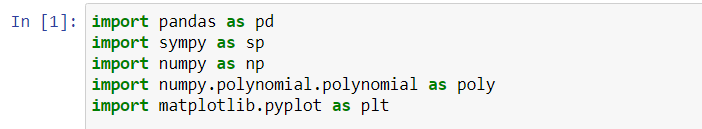
\includegraphics[width=13cm]{Img/4a1.PNG}
	\end{figure}

	Las funciones definidas fueron:
	\begin{figure}[h]
		\centering
		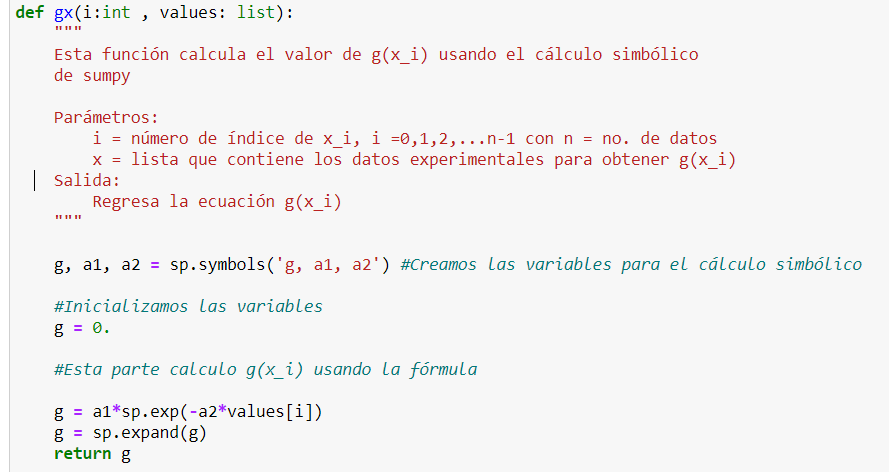
\includegraphics[width=11cm]{Img/4a2.PNG}
	\end{figure}
	\begin{figure}[h]
		\centering
		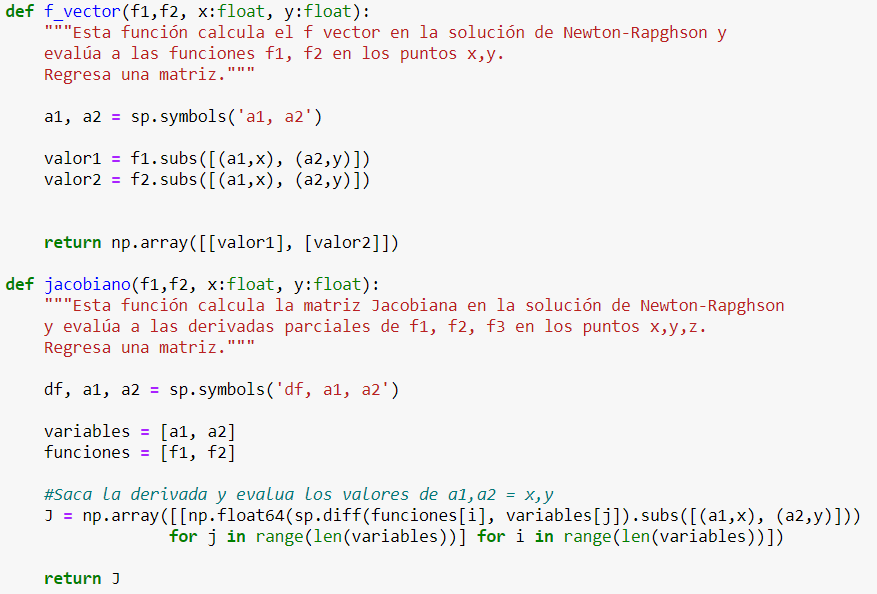
\includegraphics[width=11cm]{Img/4a3.PNG}
	\end{figure}
	
	Lo siguiente es el cuerpo del código principal el cual se encarga de estimar $a_1$ y $a_2$ por Newton-Raphson:
\newpage
	\begin{figure}[h!]
		\centering
		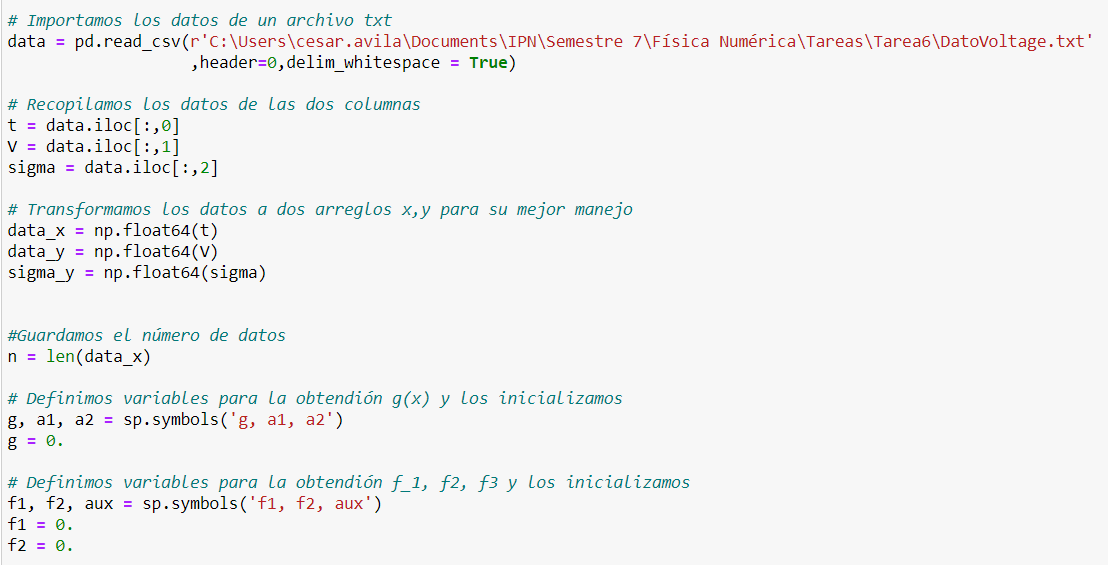
\includegraphics[width=13cm]{Img/4a4.PNG}
	\end{figure}
	\begin{figure}[h!]
		\centering
		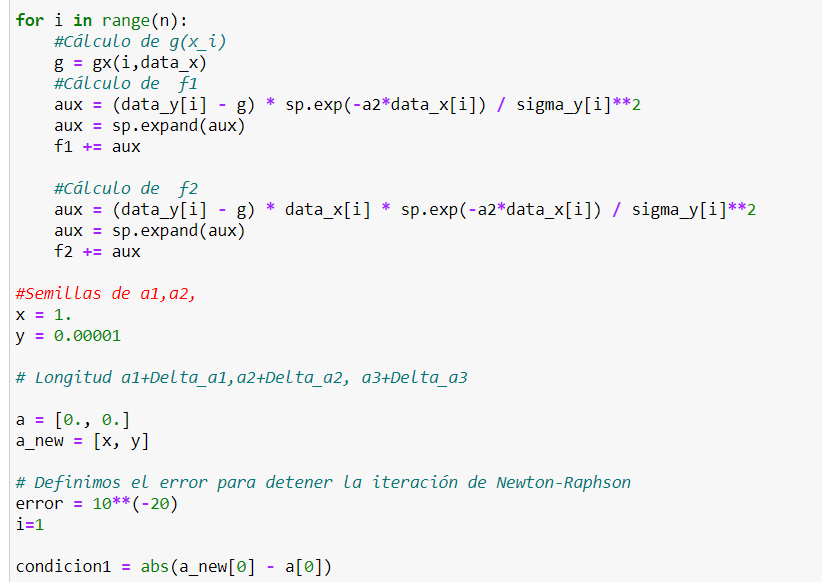
\includegraphics[width=13cm]{Img/4a5.PNG}
	\end{figure}
\newpage

	Esta parte calcula iteradamente por Newton-Raphson:
	
	\begin{figure}[h!]
		\centering
		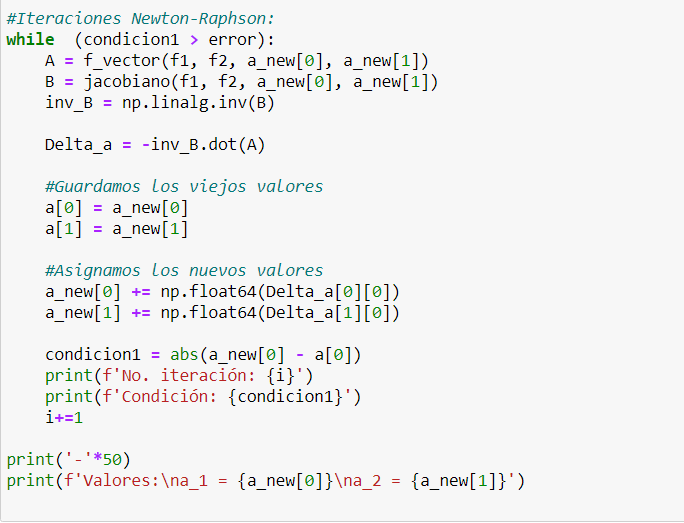
\includegraphics[width=11cm]{Img/4a6.PNG}
	\end{figure}
	
	Los resultados fueron:
	
	\begin{figure}[h!]
		\centering
		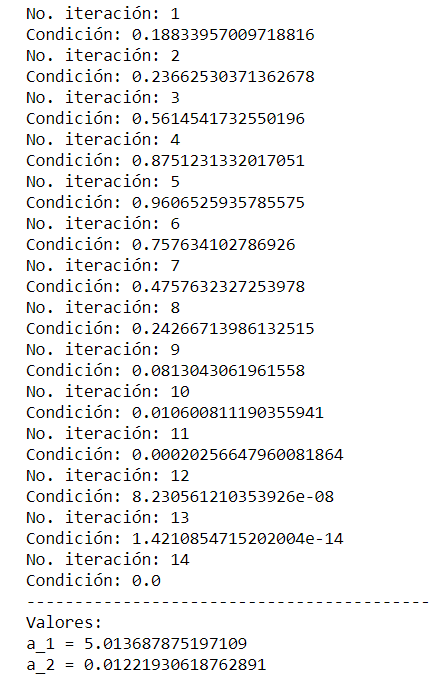
\includegraphics[width=6cm]{Img/4a7.PNG}
	\end{figure}	
	
	Por lo tanto:
	\begin{align*}
		a_1 = V_0 &= \SI{5.0136}{Volts}	\\
		a_2 = \Gamma &= 0.0122
	\end{align*}
	
\newpage
	
\begin{enumerate}
	\item [\textbf{(b)}] Encuentre el valor de $\chi^2$ para su ajuste. ¿Tiene sentido?
\end{enumerate}	
	\textit{Solución.}\\
	Recordemos que:
	$$\chi^2 = \sum_{i=1}^{16} \left[\frac{y_i - a_1 e^{-a_2 t_i}}{\sigma_i}\right]^2$$
	Donde usaremos los valores de $a_1$ y $a_2$ determinados en el ejercicio anterior. Este cálculo se realiza en el siguiente código:
	\begin{figure}[h!]
		\centering
		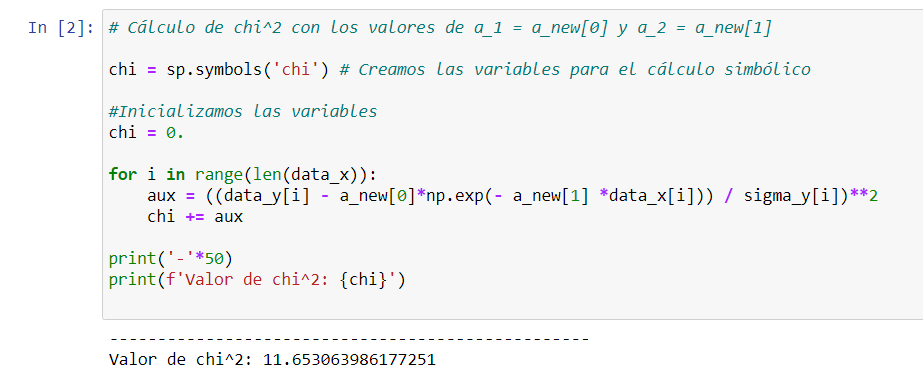
\includegraphics[width=13cm]{Img/4b1.PNG}
	\end{figure}
	
	De esa forma $\chi^2 \approx 12$, lo cual es menor a nuestro número de datos 16. Como es un valor cercano al número de datos, podemos considerarlo como un buen ajuste.
	
\begin{enumerate}
	\item [\textbf{(c)}] Realice una gráfica semi-log para los datos y el ajuste.
\end{enumerate}	
\textit{Solución.}\\	
	Notemos que de (\ref{voltaje}) obtenemos:
	$$\underbrace{\ln (V(t))}_y = \underbrace{-\Gamma}_m t +\underbrace{\ln (V_0)}_b$$
	La cual es una ecuación de la forma $y = mx + b$. Para obtener $m$ y $b$ realizaremos un ajuste de recta por mínimos cuadrados. \\
	Lo primero a realizar será obtener los valores logarítmicos y la dispersión de las incertidumbres dadas por:
	$$\sigma_y =\frac{\partial y}{\partial V} \sigma_V = \frac{\sigma_V}{V}$$
	Esto se realiza en el siguiente código:
	\begin{figure}[h!]
		\centering
		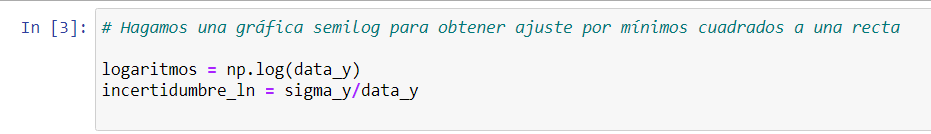
\includegraphics[width=13cm]{Img/4c1.PNG}
	\end{figure}
	
	Lo siguiente a realizar es graficar junto con las incertidumbres:
\newpage
	\begin{figure}[h!]
		\centering
		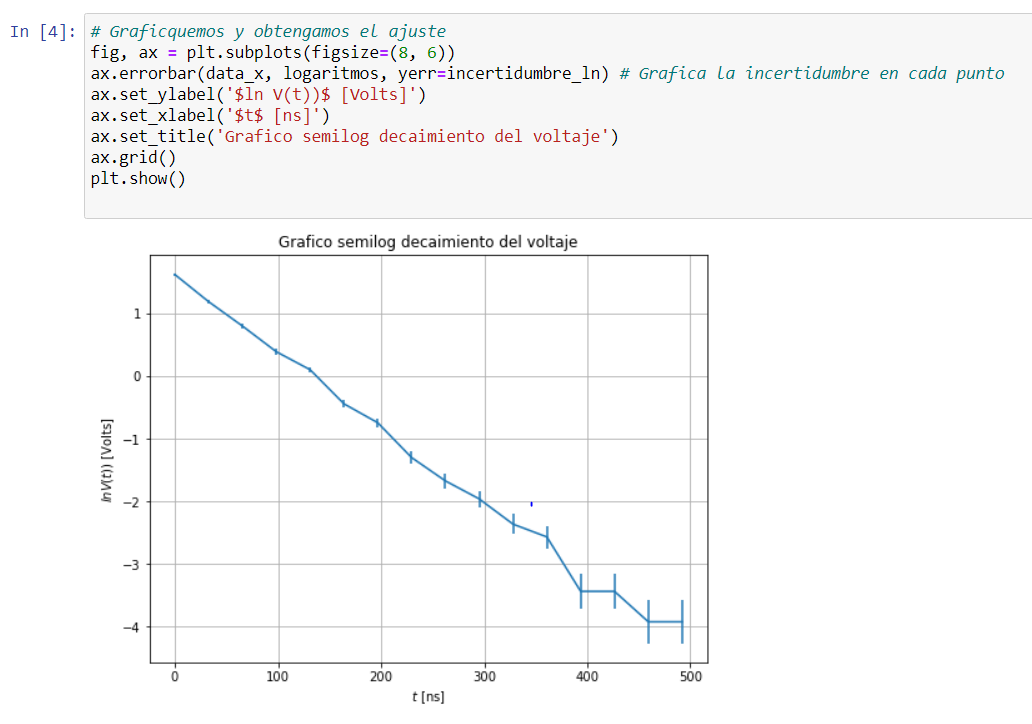
\includegraphics[width=14cm]{Img/4c2.PNG}
	\end{figure}

	Podemos ver que se tiene una tendencia lineal, por lo que realizaremos el ajuste de recta por mínimos cuadrados. En el siguiente algoritmo se realiza esta parte:
	\begin{figure}[h!]
		\centering
		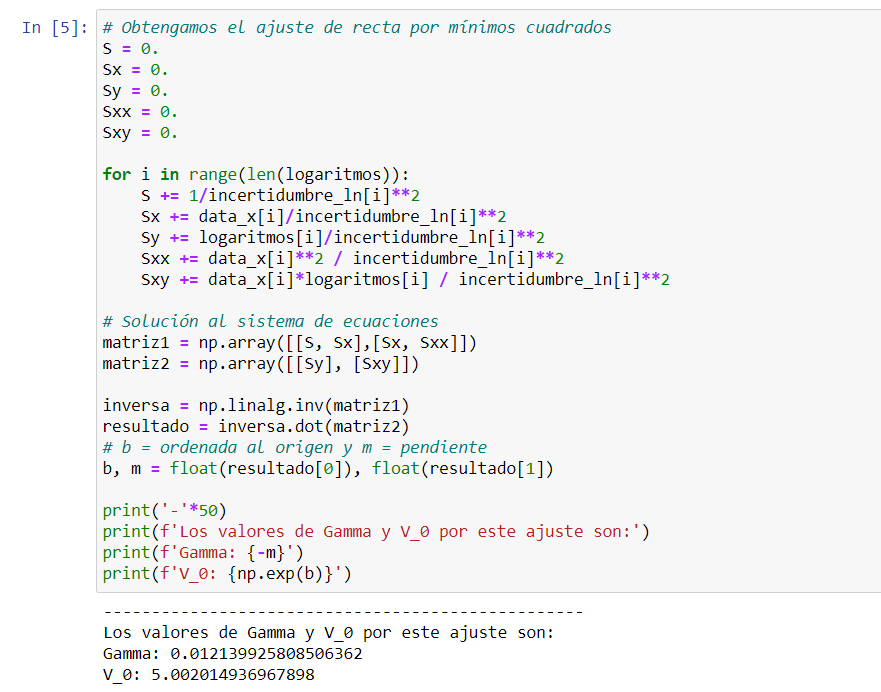
\includegraphics[width=14cm]{Img/4c3.PNG}
	\end{figure}
	
	Por lo tanto, los valores determinados por este ajuste de recta son:
	\begin{align*}
		V_0 &= \SI{5.0020}{Volts}	\\
		\Gamma &= 0.01213
	\end{align*}
	Los cuales coinciden mucho con el inciso (a).
%%%%%%%%%%%%%%%%%%%%%%%%%%%%%%%%%%%%%%%%%%%%%%%%%%%%%%%%%%%%%%%%%%%%%%%%%%%%%%%%%%%%%%%%%%%%%%%%%%%%%%%%%%%%%%%%%%%%%%%%	
\hrule
\subsection*{\textbf{5. Ajustando el espectro de un cuerpo negro}}

%%%%%%%%%%%%%%%%%%%%%%%%%%%%%%%%%%%%%%%%%%%%%%%%%%%%%%%%%%%%%%%%%%%%%%%%%%%%%%%%%%%%%%%%%%%%%%%%%%%%%%%%%%%%%%%%%%%%%%%%
	La Mecánica Cuántica inición con el espectro de radiación de un cuerpo negro de Planck:
	\begin{equation}
		I(\nu, T) = \frac{2h \nu^3}{c^2}\frac{1}{\exp(\frac{h\nu}{kT}) -1}	\label{Planck}
	\end{equation}
	donde $I(\nu,T)$ es la energía por unidad de tiempo de radiación con freceucnai $nu$ emitida en la superficie por unidad de área, por unidad de ángulo sólido y por unidad de frecuencia por un cuerpo negro a temperatura $T$. El parámetro $h$ es la constante de Panck, $c$ es la velocidad de la luz en el vacío y $k$ es la constante de Boltzmann. El proyecto COBE midió la radiación cósmica de fonde, obteniendo algunos datos experimentales.
	
\begin{enumerate}
	\item [\textbf{(a)}] Grafique los datos del COBE y vea si tienen una forma similar a la radiación de cuerpo negro dada por Planck.
\end{enumerate}
\textit{Solución.}\\
	Para graficar los datos usaremos el siguiente algoritmo, el cual se encarga de recopilar los datos en tres arreglos distintos. Note que las incertidumbres se han dividido entre 1000 con el objetivo de usar las mismas unidades de medición.
	\begin{figure}[h]
		\centering
		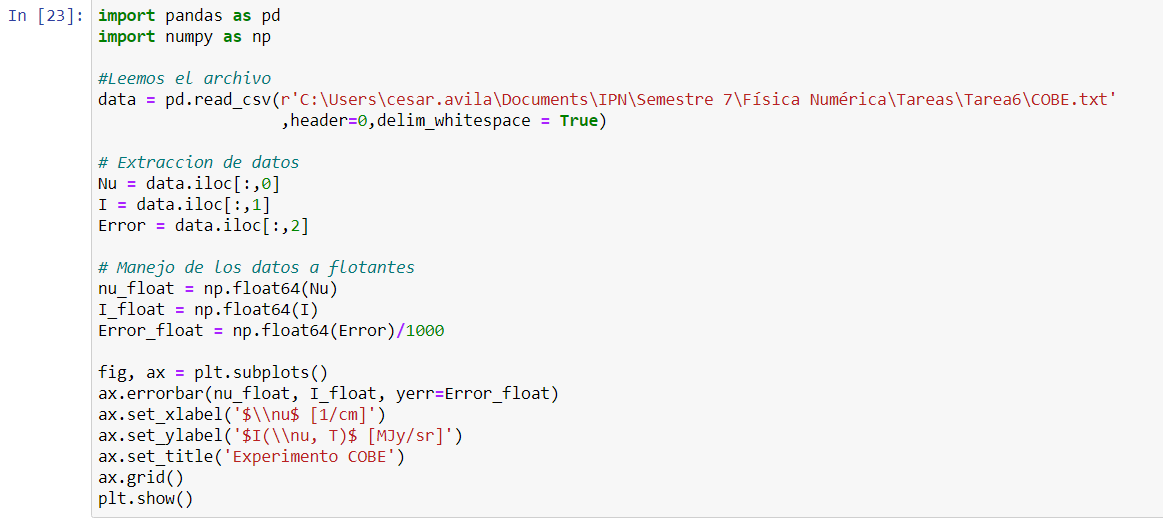
\includegraphics[width=13cm]{Img/5a1.PNG}
	\end{figure}
	
	Produciendo el siguiente gráfico:
\newpage
	\begin{figure}[h]
		\centering
		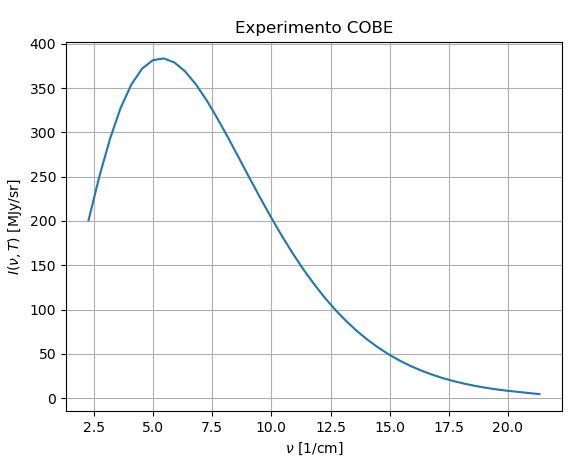
\includegraphics[width=8cm]{Img/5a2.PNG}
		\caption{Dispersión de los datos experimentales de COBE.}
	\end{figure}
	
	Por otro lado, para la radiación de cuerpo negro de Planck se tiene que:
	
	\begin{figure}[h]
		\centering
		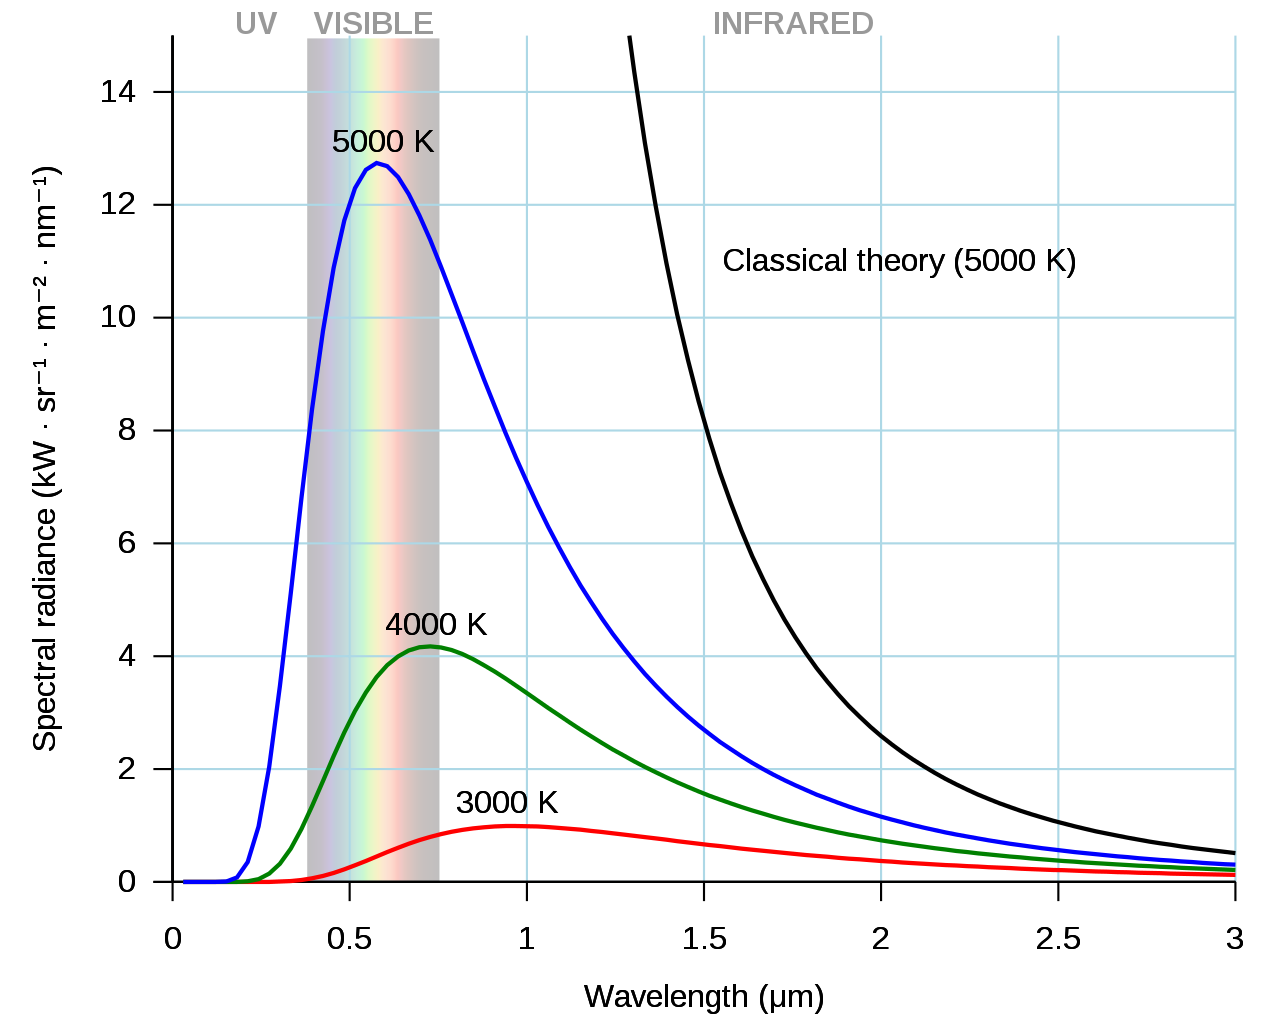
\includegraphics[width=8cm]{Img/Planck.PNG}
		\caption{Radiación de cuerpo negro de Planck.}
	\end{figure}
	
	Podemos ver que la dispersión de los datos de COBE tienen la misma forma que la radiación de cuerpo negro de Planck.
	
\begin{enumerate}
	\item [\textbf{(b)}] Utilice estos datos para estimar la temperatura $T$ de la radiación cósmica de fondo, ajustando la curva por mínimos cuadrados.
\end{enumerate}
\textit{Solución.}\\
	Para realizar el ajuste, de la ecuación (\ref{Planck}) la modificaremos de forma que podamos obtener un ajuste lineal. La expresión obtenida es:
	\begin{equation}\label{lineal}
		\underbrace{\ln \left(\frac{2h}{c^2}\frac{\nu^3}{I}+1\right)}_y = \frac{1}{T}\underbrace{\frac{h\nu}{k}}_x
	\end{equation}
	Esta ecuación es de la forma $y = a x$. Nuestro objetivo será determinar la pendiente $a = \frac{h}{kT}$ para poder determinar el valor de $T$.\\
	Lo primero que haremos será definir las constantes y hacer las conversiones adecuadas. Usaremos unidades del SI. De esa forma:
	\begin{align*}
		 h &= \SI{6.6261e-34}{J\cdot s}\quad\text{(Cte. de Planck)}	\\
		 c &= \SI{2.9979e8}{m/ s}\quad\text{(Vel. de la luz)} 	\\
		 k &= \SI{1.3806e-23}{J/ K}\quad\text{(Cte. de Boltzmann)}
	\end{align*}
	Por otro lado, las unidades Jansky (Jy) están definidas de la siguiente forma:
	$$\SI{1}{Jy} = 10^{-26} \frac{\si{W}}{\si{m^2 \cdot Hz}}$$
	De esa forma, las mediciones para la irradiancia cuyas unidades son [MJy/sr] deberán multiplicarse por un factor de $\num{1e-20}$ para tener unidades del SI. Por otro lado, notemos que las mediciones para $\nu$ tienen como unidad [1/cm]. Esto se debe a que en ocasiones la frecuencia se toma como $\nu = \frac{1}{\lambda}$ donde $\lambda$ es la longitud de onda. Para modificarlo y tener a la frecuencia en [Hz] tal y como la conocemos, recordemos que $\nu = \frac{c}{\lambda}$. De esta forma, si nuestra medición dice que tenemos $\nu = \SI{10}{(cm)^{-1}}$ en realidad tenemos $\nu = c_{cgs}\cdot \SI{10}{Hz}$, donde $c_{cgs} = \SI{2.9979e10}{cm/s}$ (Vel. de la luz en cgs).\\
	En las siguientes lineas de código realizamos este cambio:
	\begin{figure}[h]
		\centering
		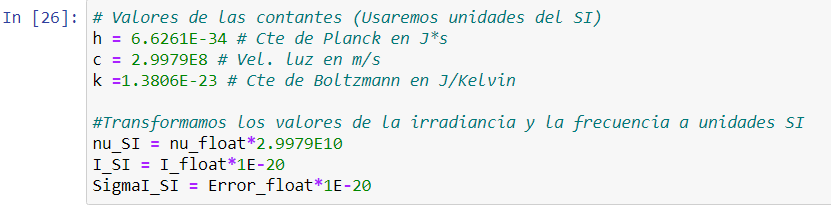
\includegraphics[width=13cm]{Img/5b1.PNG}
	\end{figure}
	
	Lo siguiente a realizar será crear tres listas: \texttt{logaritmos},\texttt{ incertidumbres\_ln} y \texttt{eje\_x}. En la lista \texttt{logaritmos} guardaremos los valores de $y$ de la ecuación (\ref{lineal}) para el ajuste lineal, en \texttt{eje\_x} guardaremos los valores de $x$. Por último, en \texttt{incertidumbres\_ln} guardaremos los valores de la dispersión de las incertidumbres usando la siguiente fórmula:
	$$\sigma_y = \left|\frac{\partial y}{\partial I}\right| \sigma_I = \frac{\frac{2h\nu^3}{c^2 I^2}}{\frac{2h}{c^2}\frac{\nu^3}{I} + 1}$$
	Para guardar los valores en estas tres listas se utilizó un ciclo \texttt{for} tal como se aprecia en la siguiente imagen:
	\begin{figure}[h]
		\centering
		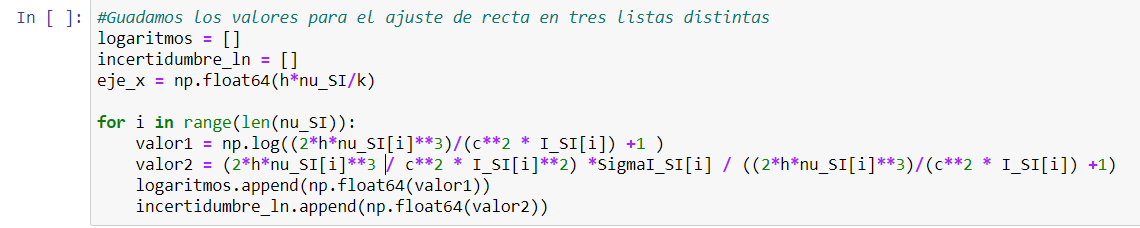
\includegraphics[width=16cm]{Img/5b2.PNG}
	\end{figure}
	
	Con estos valores ya podremos realizar un ajuste lineal. Para ver la tendencia de los datos, grafiquemos $y$ vs $x$ (\texttt{logartimos} vs \texttt{eje\_x}). 
\newpage
	\begin{figure}[h]
		\centering
		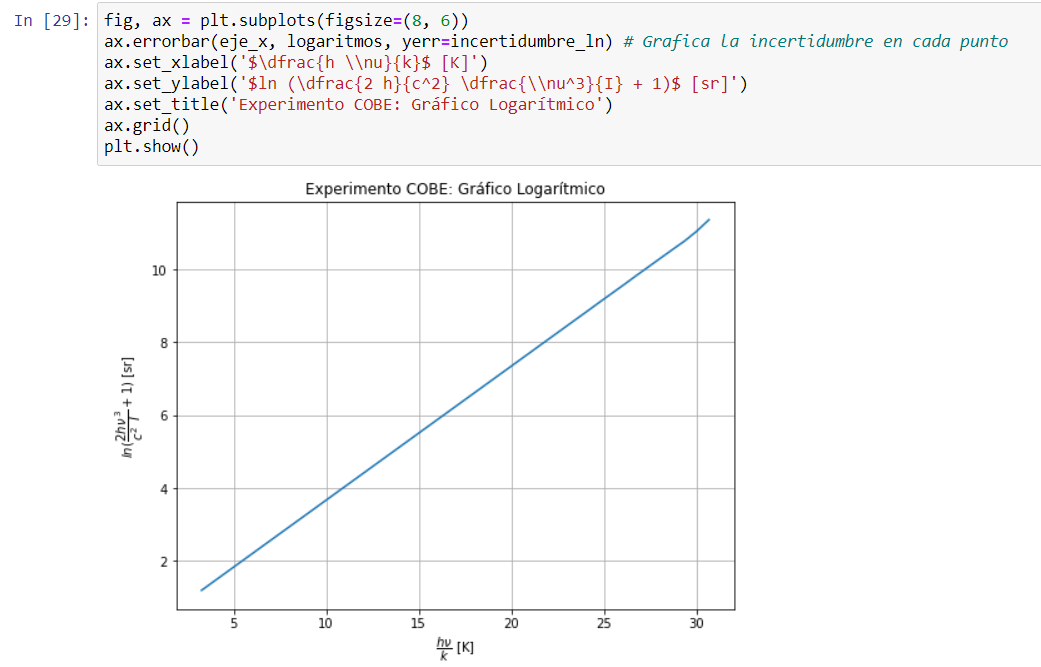
\includegraphics[width=15cm]{Img/5b3.PNG}
	\end{figure}
	
	Podemos ver que la tendencia es lineal, por lo que será posible realizar un ajuste por mínimos cuadrados. DE la teoría sabemos que el ajuste propuesto es de la forma:
	$$g(x) = a_1 + a_2 x$$
	Determinaremos $a_1$ y $a_2$. De esta forma la temperatura buscada es $T=1/a_2$. Para ello requeriremos obtener $S,S_x, S_y, S_{xx}$ y $S_y$ tal y como se definieron en clase. En la siguiente parte de código se realiza esta parte:
	\begin{figure}[h]
		\centering
		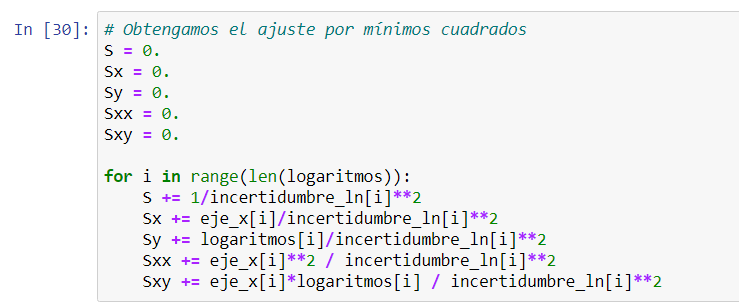
\includegraphics[width=12cm]{Img/5b4.PNG}
	\end{figure}
	
	Con estos valores recordemos también que se tienen el siguiente sistema de ecuaciones:
	\begin{align*}
		S_y - S a_1 -S_x a_2	&= 0	\\
		S_{xy} -S_x a_1 -S_{xx} a_2 &= 0
	\end{align*}
	De forma matricial:
	$$\left[ {\begin{array}{cc}
			S & S_x \\
			S_x & S_{xx} \\
	\end{array} } \right] \left[ {\begin{array}{c}
	a_1   \\
	a_2   \\
\end{array} } \right]	= 
  \left[ {\begin{array}{c}
		S_y  \\
		S_{xy}  \\
\end{array} } \right]
$$

	Basta despejar la segunda matriz para obtener los valores de $a_1$ y $a_2$. Esto se realiza en el siguiente código:
	
	\begin{figure}[h]
		\centering
		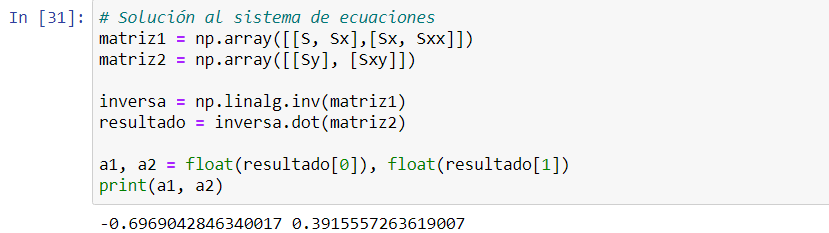
\includegraphics[width=13cm]{Img/5b5.PNG}
	\end{figure}
	
	Por lo que la temperatura resultante es:
	\begin{figure}[h]
		\centering
		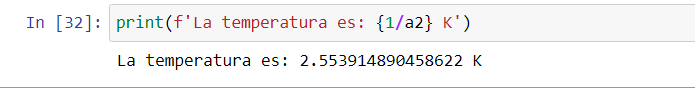
\includegraphics[width=10cm]{Img/5b6.PNG}
	\end{figure}
	
	
\end{document}